\documentclass[13pt,a4paper]{article}
\usepackage[utf8]{inputenc}
\usepackage[english]{babel}
\usepackage{amsmath}
\usepackage{amsfonts}
\usepackage{amssymb}
\usepackage{graphicx}
\author{Alejandro García Peláez}
\title{EOS Documentation}
\begin{document}

\maketitle 
\begin{center}
Offline version
\end{center}

\break

\vspace*{7cm}
\noindent\begin{flushleft}
 \footnotesize{This work is licensed under the Creative Commons Attribution 4.0 International License. \newline To view a copy of this license, visit http://creativecommons.org/licenses/by/4.0/.}
\end{flushleft}

\break

\vspace*{-3cm}
\section*{Strandbeest Mechanism}

The Jansens Linkage, is an eleven-bar mechanism designed by Theo Janssen who studied physics at the Delft University of Technology but he left the university without a degree; the first "Strandbeest" that the autor created was in 1990, which are moving kinetic structures (wind-propelled).

\noindent\newline The mechanism has some parts in order to get the recognized movement. It can be see in the next picture: \newline \newline

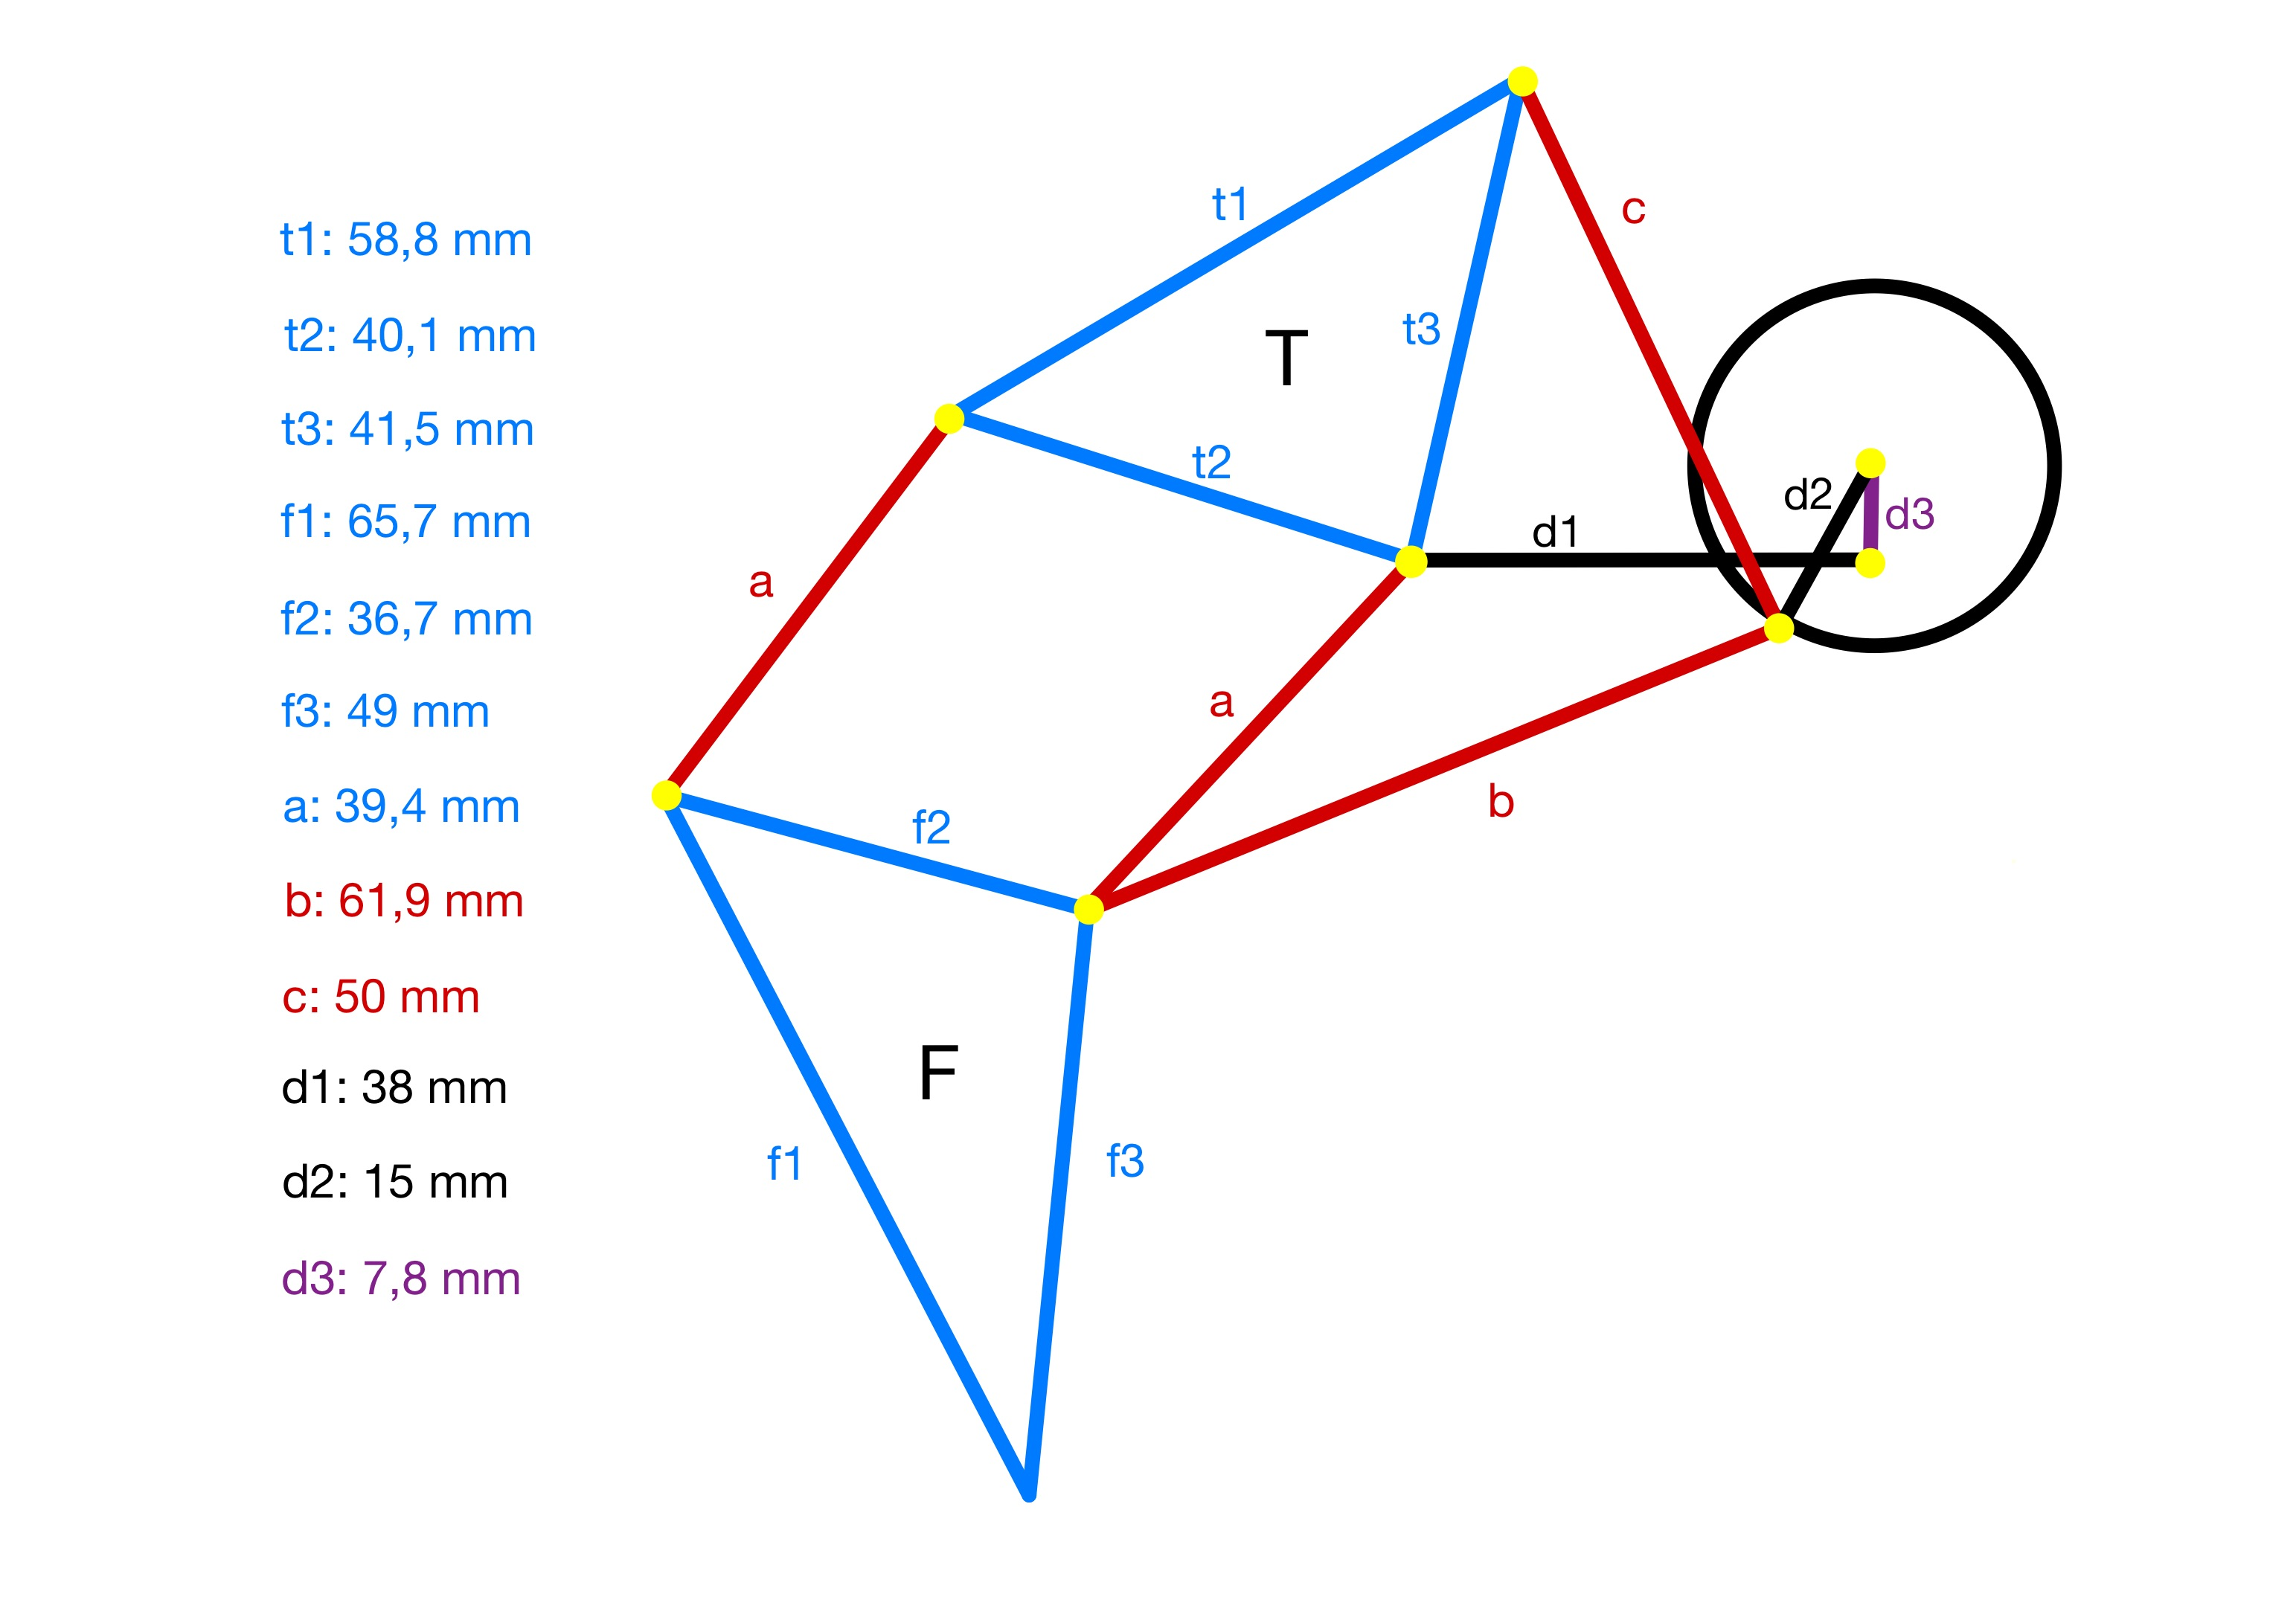
\includegraphics[scale=0.1]{"project_pictures/measures.jpg"}


We are going to use gears instead of an eleven bar.

\section*{Electronic}

EOS intends to encourage anyone who has an interest to build their own version of the project; That is why there is no permanent description of electronic materials since the limit is one's own imagination and creativity. \newline

\noindent We just need a couple of geared motors and a battery to power them... and EOS will be able to walk. \newline

\begin{center}
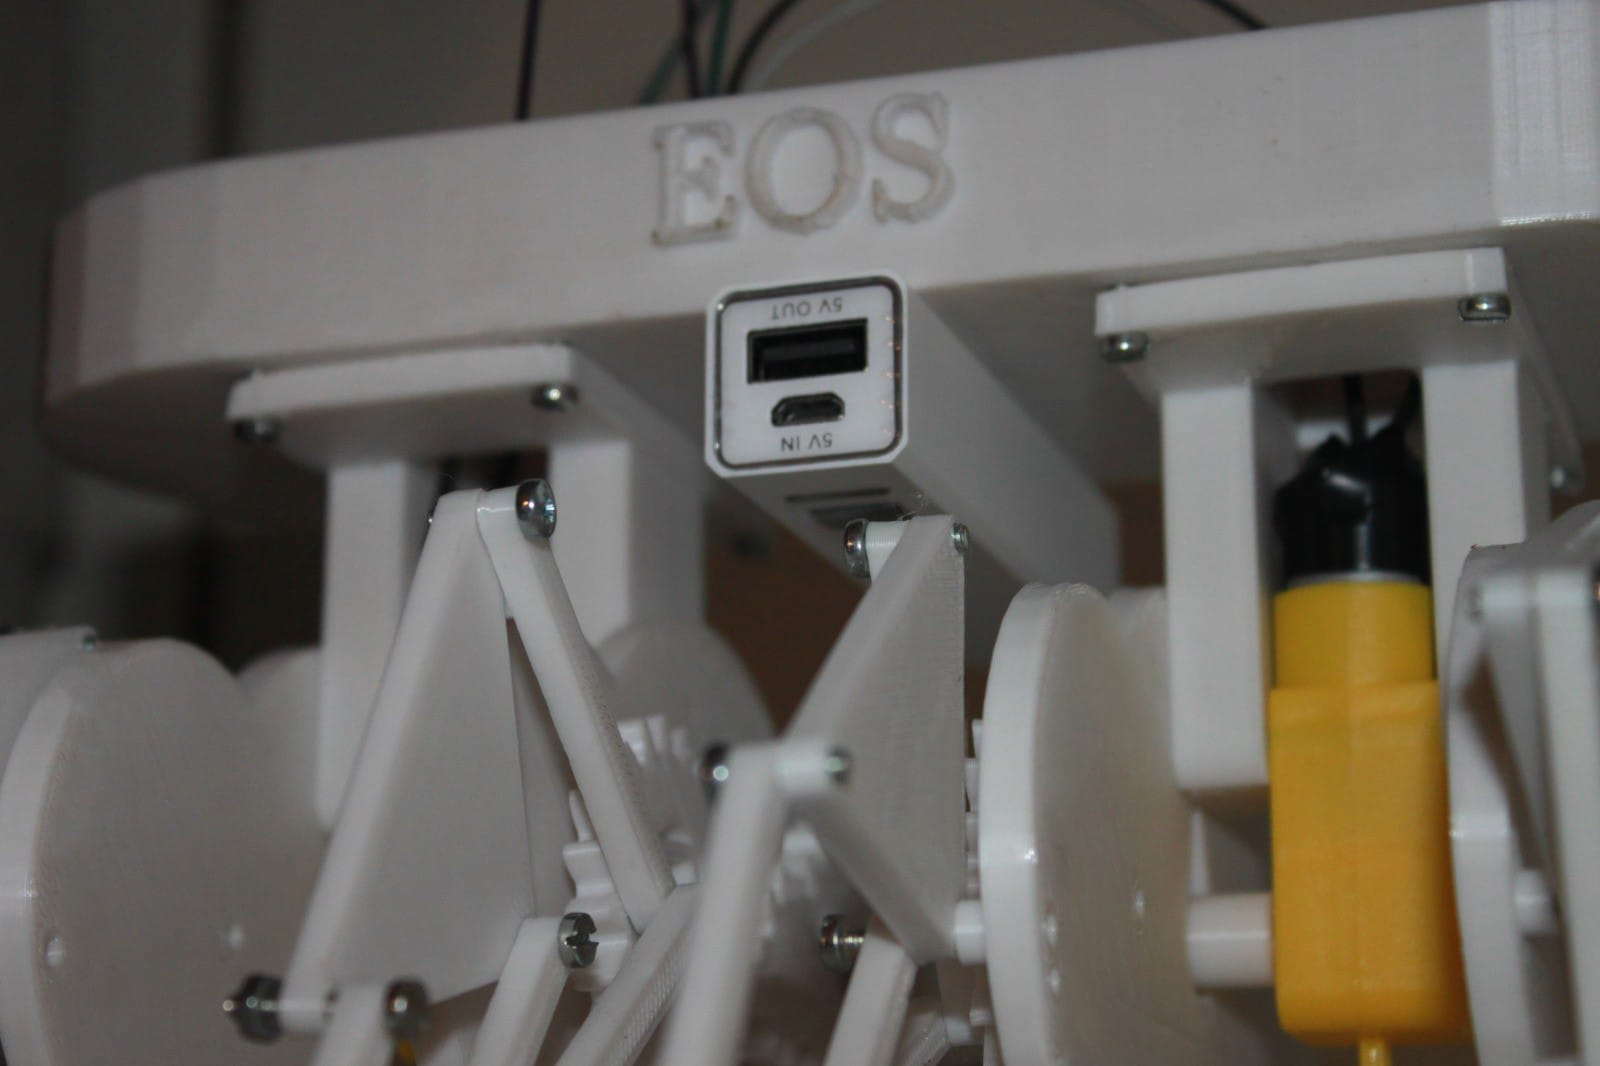
\includegraphics[scale=0.15]{"project_pictures/eos_v1_0.jpg"}
\end{center}


\end{document}